\documentclass{home_assignment}
\usepackage[defernumbers=true]{biblatex}

\DeclareBibliographyCategory{cited}
\AtEveryCitekey{\addtocategory{cited}{\thefield{entrykey}}}

\addbibresource{citation.bib}
\nocite{*}
\renewcommand\thesubsection{\Alph{subsection}.}
\begin{document}
\titlePage{Computer Networks Assignment \#2}{September 30,2020}{Sharad Kumar Ghimire}
\problem{What is guided transmission media? Explain the different guided transmission media with their features.}
A transmission media is simply the means by which data or communication signals are sent from one system to another system, i.e.  from a sender to a receiver.  If a physical link exists between the two systems, then the transmission media is called a guided transmission media. A physical path for the transmission of data is inherently provided by the guided transmission media such that the signals travelling across them are directed and contained within the physical bounds of the linkage. A simpler and more practical application of such transmission media can be found in connections between an ISP and a client. For example, a household router that’s linked to say, the Vianet/Worldlink ISP in Nepal has an optical fiber as the connection medium. This means that the signal between the local router and ISP travels through the optical fiber and hence is guided within the physical bounds of the medium.
\\The various guided transmission media are discussed below:
\subsection*{Twisted Pair Cable}
A twisted pair cable is the most basic form of a guided transmission media that, as the name suggests, contains a pair of conductors intertwined together. The spiral pattern that exists in a twisted pair actually has an importance since it cancels the electromagnetic interference resulting from some external sources. Despite being one of the oldest forms of transmission media, a twisted pai cable still ranks as one of the most common forms of guided media. This type of cable is dominantly used in house-hold or office usage for LANs and for telephone networks. A twisted pair cable can be further categorized into two sub-groups:
\subsubsection*{Unshielded Twisted Pair Cable}
Generally referred to as the UTP cable, it lacks the metallic shield around the copper conductor pair. The pairs are however insulated in a plastic wrap but it’s basic usage is just the color decoding for recognition. An UTP is obviously suspectable to interference due to the lack of the metallic shield, but the interference from peer cables is minimized by the twisted nature of the pair. Separate wiring of different signals as in ethernet cables allows for easier installation and efficient cable usage.
\subsubsection*{Shielded Twisted Pair Cable}
Unlike its unshielded counterpart, the STP cable consists of a metallic shielding around the twisted pair hence giving it more leverage for a lengthier connection with faster data rate and less electromagnetic interference. Since the STP cable uses the shield as a ground connection to get rid of the noise, the connection is very important otherwise, its main functionality is worthless. It is much costlier than the UTP cable and much thicker in size making it less flexible.\\ STP cable is available in mainly three forms of shielding,
\begin{itemize}
\item All the pairs collectively having a shield
\item Each pair having seperate foil shielding
\item Each pair having a shield along with another shield for the overall wires 
\end{itemize}
\cite{yang} interprets some key aspects regarding the features of a twisted pair cable.
\begin{figure}[H]
\centering
\includegraphics[scale=0.75]{./Figures/twisted.jpg}
\caption{STP and UTP cables taken from \cite{twisted}}
\label{fig:twisted}
\end{figure}
\subsection*{Coaxial Cable}
A coaxial cable has two copper conductors but unlike the twisted pair cable, the conductors are concentrically arranged, hence the name coaxial. Generally, a single interior wire is surrounded by a hollow cylindrical conductor which itself is insulated. There is a shielding, usually by a metallic foil such that it acts as the second conductor and a noise canceling shield. This type of cable is generally used for cable television transmission and LANs as well.\\
\begin{figure}[H]
\centering
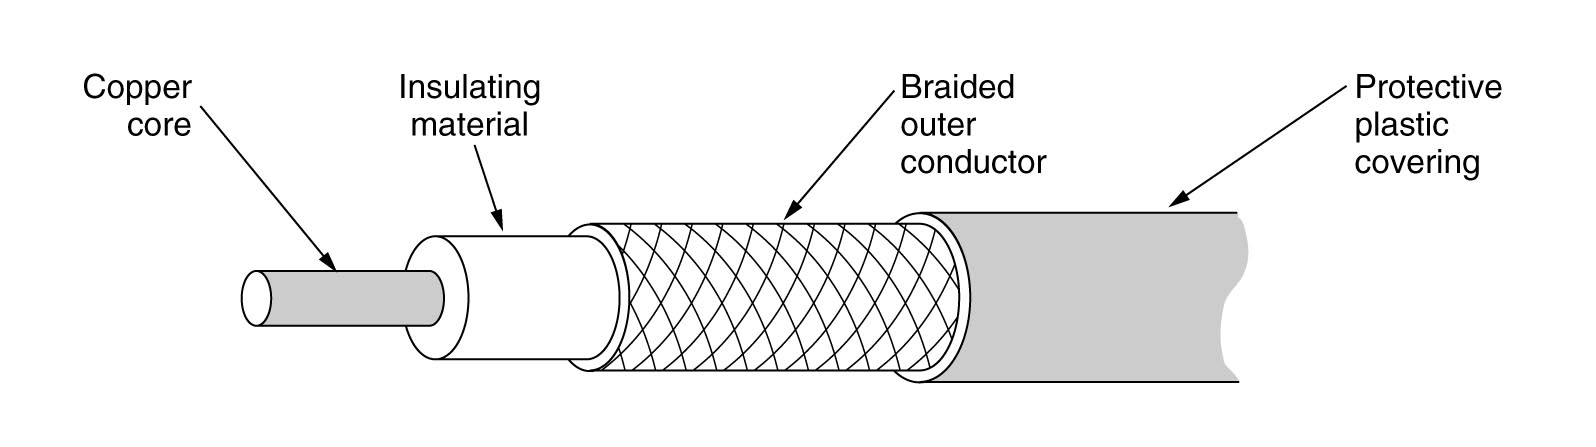
\includegraphics[scale=1]{./Figures/coaxial.jpg}
\caption{Co-axial cable taken from \cite{coaxial}}
\label{fig:coaxial}
\end{figure}
One of the better usages of a coaxial cable is that it can be used as a shared medium, i.e., multiple end systems can be directly connected to the cable, like in a bus topology. A practical sight of this could be recalled when television channel transmission in Nepal was carried out with coaxial cables, since multiple users would be able to connect to the same cable line through connectors.
\subsection*{Optical Fiber Cable} 
An optical fiber cable is essentially the transmission media used for fiber optics technology which uses light to transfer data and signals. Presence of a light pulse indicates the high bit whereas its absence indicates the low bit. A source of light generates the pulsating light that travels through the optical cable’s glass core following total internal reflection, and is decoded in the destination end by means of light detectors. An optical fiber cable can be thought to be similar in construction to a coaxial cable where the major differences being the glass core instead of the copper conductor and the necessity of a shield.\\An optical fiber cable is starting to dominate long route transmissions and high-speed internet access say the Fiber to Home initiative all around the world. There are basically two ways in which the light can traverse through the cable. If the light follows total internal reflection within the core essentially providing different modes to each ray, then the media is called multimode fiber. Likewise, if the diameter of the cable is reduced such that it is nearabout few wavelengths of the light, then the rays travel in a straight path without total internal reflection and hence are said to be in single-mode fiber.
\begin{figure}[H]
\centering
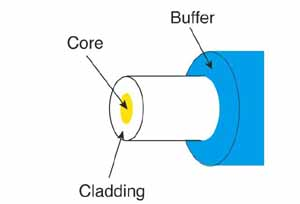
\includegraphics[scale=1]{./Figures/optical.jpg}
\caption{Optical fiber cable taken from \cite{optical}}
\label{fig:coaxial}
\end{figure}
\problem{What is switching? What is the importance of switching in a communication system?}
Data or signal that is being transmitted from the source to a destination needs a path to travel, no matter the media used. Switching is simply the technique or procedure based on which packets are forwarded towards the destination from one port to another. Port can be thought of the landmarks the packet passes while on-route to its destination. A port forwards the packets towards the destination and essentially switches the control. Nodes or ports are the simple redistribution points that receive as well as forward data to other nodes.\\Switching can be broadly divided into three types:
\subsubsection*{Circuit Switching}
\begin{itemize}
\item Such type of network contains multiple switches that actually change the physical linkage between two nodes.
\item Before the communication over the line starts, the nodes take reservation for the available resources and a pre-specified route is used such that no other data is permitted through it, hence making it a reliable switching method.
\item Once a proper connection between two endpoints is established, a dedicated transfer path remains between the two until the communication terminates.
\item Resource may be wasted while using this technique.
\item This form of switching is most widely used in telephone networks where the dialer and receiver first establish a connection route, then transfer the data, and disconnect once they're done.
\end{itemize}
\begin{figure}[H]
\centering
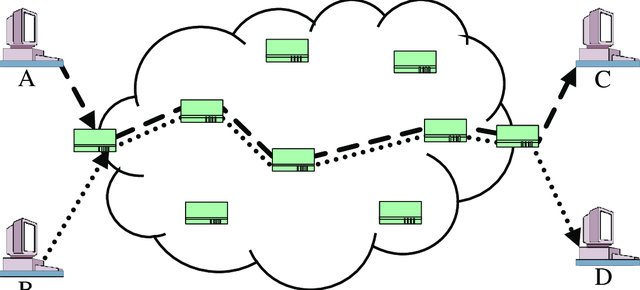
\includegraphics[scale=1.5]{./Figures/cktswitching.jpg}
\caption{Circuit Switching taken from \cite{cktswitching}}
\label{fig:cktswitching}
\end{figure}
\subsubsection*{Packet Switching}
\begin{itemize}
\item The overall messages are divided into different packets with either fixed or variable sizes.
\item Resources aren't allocated for individual packets, rather the allocation occurs on demand with the first-come first-serve method.
\item Each of the endpoints consist of a temporary packet storage, also called buffer storage.
\item Size of packet depends on the network and its protocol.
\end{itemize}
\begin{figure}[H]
\centering
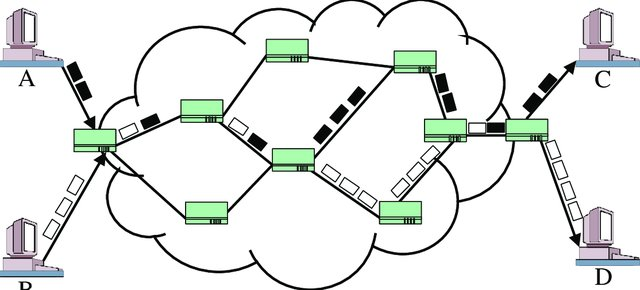
\includegraphics[scale=1.5]{./Figures/pktswitching.jpg}
\caption{Packet Switching taken from \cite{pktswitching}}
\label{fig:pktswitching}
\end{figure}
\subsubsection*{Message Switching}
\begin{itemize}
\item In this form of switching, the overall message is regarded as a single unit and is transfered without packeting.
\item Each node has a buffer that stores the message until an appropriate hop forward is available. A hop is simply the transfer of the message from one node to another towards the destination. 
\item All the nodes in the transfer path must have sufficient buffer to store the whole message.
\item This form of switching introduces large queuing delay.
\item Since it isn't suitable for streaming videos and audios, this method is obsolete.
\begin{figure}[H]
\centering
\includegraphics[scale=0.75]{./Figures/msgswitching.png}
\caption{Message Switching taken from \cite{msgswitching}}
\label{fig:msgswitching}
\end{figure}
\end{itemize}
An unswitched network model would require maximum data lines since every port must be physically connected. But switching a network provides for the minimum usage of actual physical linkage between the ports hence establishing an effective network.Some of the importance of switching are:
\begin{itemize}
\item A network switch can connect devices like computer and APs to the best resulting path hence better managing the network traffic.
\item LANs are divided into multiple collision domains hence increasing the LAN bandwidth.
\item Switches can connect multiple hosts without the need of physical connection between them.
\end{itemize} 
\problem{Discuss briefly on:}
\subsection{Bandwidth}
Bandwidth is the theoretical measure of the amount of data that a network can move from the source to destination in a certain frame of time. The common units of its measure are bps, Mbps or Gbps. Bandwidth of a network defines how much data can be sent over the network in ideal situations.
\subsection{Throughput}
Throughput is the actual measure of the data that a network successfully moved from the source to destination in a given time period. It’s units of measurement are alike Bandwidth measurement. An essential note about throughput and bandwidth is that, throughput can never be greater than the bandwidth of a network since a network can never successfully transmit more data than the bandwidth limits of the system.
\subsection{Delay}
Delay is defined as the time needed by a packet of data to reach from one endpoint of a network to another. Simply put, delay is the time that a packet needs to travel its entire path. Delays in a network occur mainly due to the following causes,
\subsubsection*{Processing Delay}
As the name suggests, it is the delay that occurs due to the processing time of the routers to determine the forward path of the packet, or check the header values.
\subsubsection*{Queuing Delay}
This type of delay is the time for which a packet of data is enqueued and waiting until the network is busy transferring another packet.
\subsubsection*{Propagation Delay}
This is the time required for a packet or bit of data to travel along the medium. It is dependent on the characteristics of the transmission media and its length.
\subsubsection*{Transmission Delay}
This type of delay is the time needed to push all the bits onto the transmission medium. It depends on the no. of bits and transmission rate.
\subsection{Latency} Latency is the time that a packet takes to be sent over the network from source to destination. In simple words, latency can be thought of as the round-trip delay for a network. A term most commonly used to describe latency is the ping of a network.   Ping is the signal sent over the network to check the latency.   It measures the time delay between the transmission of packets of data over a network with the receiving of those packets. The devices that the packet uses to hop to the destination also introduces additional latency. The major determining factor of high latency network is the geographical distance between the two endpoints. For example, a server in India would have less latency for a request from Nepal than that located in USA under similar circumstances.
\subsection{RTT}
RTT, abbreviation of Round-Trip Time is the time that a packet takes to complete a round trip between the end points, meaning that from source to destination and back to the source. For smaller distance transmissions, latency can define the RTT of a network, but in more complex scenarios, latency can only give an idea about the RTT delay rather than completely define it.
\subsection{ISDN}
ISDN, abbreviation for Integrated Services Digital Network is the predefined standard for voice and data transfer over the digital networks. With a maximum speed of 128 kbit/s, the ISDN standard allows for two calls to take place parallelly.
\setcounter{subsection}{0}
\problem{Differentiate between:}
\subsection{FDM vs. TDM}
\difference{FDM}{TDM}{Abbreviation              & Frequency Division Multiplexing                                             & Time Division Multiplexing                                                                           \\
    \hline
    Functioning Mechanism      & Divides the channel into multiple frequency ranges without overlaps.        & Divides and allocates different time periods to each channel.                                        \\
    \hline
    Flexibility and efficiency & Can't change the allocated frequency dynamically, hence are less efficient. & Can dynamically allocate more time for signals depending on their bandwidth and hence are efficient. \\
    \hline
    Latency                    & Since signal can be transmitted any time, latency is reduced significantly. & Since only one channel transmits at a time, queuing delay is dominant resulting in higher latency.   \\
    \hline 
    Requirements               & Guard band is a must.                                                & Synchronization pulse is needed.                                                                     \\
    \hline
    Types of signals used      & Analog signal                                                               & Analog and Digital signal                                                                            \\
    \hline}
    \vspace{-0.1in}
\subsection{Circuit switching vs. Packet switching}
\difference{Circuit switching}{Packet switching}{Path formation                     & Data units know the entire path address and is established before transfer.                           & Data units(packets) only know the final address since the overall path is decided by the routers dynamically. \\ \hline
    Phases                             & First connection is established, then data is transferred and finally connection is terminated.       & Data transfer takes place directly.                                                                           \\ \hline
    Data processing                    & Occurs at source.                                                                                     & Occurs at all intermediate nodes.                                                                             \\ \hline
    Delay and reliability              & Delay is fairly uniform and hence this is a reliable switching technique.                             & Delay between packets isn't uniform and hence isn't reliable.                                                 \\ \hline
    Resource reservation and bandwidth & Since path is fixed for a transfer, resource is reserved for a transfer and hence bandwidth is fixed. & No resource allocation resulting in dynamic bandwidth.                                                        \\ \hline
    Packet recording                   & Not possible since it isn't a store and forward technique.                                            & Possible since it is a store and forward technique.                                                           \\ \hline}
\subsection{Datagram vs. Virtual Circuit switching}
\difference{Datagram}{Virtual Circuit}{Path                   & Data packets are free to decide the dynamic path as per the routers.                                                  & Transmission path is predetermined such that all the packets use the same path following the first one.                                                                                        \\ \hline
    Connection type        & Connection less since reservation of resource doesn't take place. This is the form of a true packet switching method. & Connection oriented since reservation of resources occurs for fixed bandwidth similar to a circuit switching method. Not a pure connection-oriented service, rather a virtual link is created. \\ \hline
    Headers                & Each data packet must have a separate header for recombination at the destination. & Only the first packet needs to have a header because of the common path the packets take. \\ \hline
    Arrival and reordering & Data packets arrive randomly and are sorted as per the header information.                                            & Data packets arrive in sequence and don't need additional processing.                                                                                                                          \\ \hline
    Re-connection          & In case of a data link disconnection, transfer can continue without restarting.                                       & Transfer has to be started again if a link is down.                                                                                                                                            \\ \hline
    Cost                   & Cheaper as compared to virtual circuits.                                                                              & Expensive in installation and maintenance.                                                                                                                                                     \\ \hline}
    \pagebreak
\printbibliography[heading=bibintoc,title={Bibliography}, category=cited]
\printbibliography[heading=bibintoc,title={Additional References},notcategory=cited]
\end{document}